\chapter{Prerequisiti di Algebra}

Prima di iniziare a trattare gli argomenti principali del corso,
è necessario ripassare alcuni concetti di algebra alla base della teoria dei codici introducendone alcuni nuovi.

In particolare questo capitolo si concentra sulle strutture algebriche di semigruppi e monoidi e di loro proprietà utili per la teoria dei codici.

Inizialmente però, per addentrarci nelle definizioni delle suddette strutture algebriche, è necessario introdurre alcune notazioni preliminari, che verranno conservate per tutto il corso di questi appunti.

\section{Nozioni Preliminari}

Le lettere maiuscole \(A, B, X, Y \ldots\) indicheranno generalmente insiemi, che siano finiti o infiniti.
Per quanto riguarda gli insiemi numerici tradizionali, useremo:
\begin{itemize}
  \item \(\N = \set{0,1,2,\ldots}\) per i numeri naturali (incluso lo zero);
  \item \(\N_+ = \set{1,2,3,\ldots}\) per i numeri naturali positivi (escluso lo zero);
  \item \(\Z\) per i numeri interi;
  \item \(\Q\) per i numeri razionali;
  \item \(\R\) per i numeri reali.
\end{itemize}
Con eventuali notazioni aggiuntive a pedice per indicare sottoinsiemi particolari (ad esempio \(\R_{\geq 0}\) per i numeri reali non negativi).

Per ogni insieme \(X\), \(\mathcal{P}(X)\) denota l'insieme delle parti di \(X\), ovvero l'insieme di tutti i sottoinsiemi di \(X\) e \(\#X\) la sua cardinalità.
Gli elementi di tali insiemi saranno indicati con le lettere minuscole corrispondenti \(a,b,x,y \ldots\), in particolare con la lettera \(n\) a indicare un generico elemento naturale se non specificato diversamente.

\section{Semigruppi e Monoidi}
\begin{definition}[Semigruppo]
  Un \keyword{semigruppo} è una coppia \((S, \cdot)\) dove \(S\) è un insieme non vuoto e \(\cdot : S \times S \to S\) è un'operazione binaria associativa, ovvero:
  \[\forall a,b,c \in S, (a \cdot b) \cdot c = a \cdot (b \cdot c).\]
\end{definition}

Questa struttura algebrica è molto generica, imponendo solo l'associatività dell'operazione binaria.
Un esempio di semigruppo è dato da \((\N',+)\) dove l'operazione binaria è la somma tra numeri naturali positivi ordinaria.

\begin{definition}[Monoide]
  Un \keyword{monoide} \((M,\cdot,1_M)\) è un semigruppo \((M, \cdot)\) dotato di elemento neutro \(1_M\) per l'operazione binaria\footnote{Denotato semplicemente \(1\) in caso di non ambiguità del monoide di riferimento}, ovvero:
  \[\forall a \in M, a \cdot 1_M = 1_M \cdot a = a.\]
\end{definition}

\begin{example}
  \begin{itemize}
    \item \((\N, +)\) è un monoide con elemento neutro \(0\).
    \item \((\N, \cdot)\) è un monoide con elemento neutro \(1\).
    \item Dato \(T\) insieme, sia \((\mathcal{P}(T), \cup, \emptyset)\) che \((\mathcal{P}(T), \cap, T)\) sono monoidi.
  \end{itemize}
  Gli esempi precedenti sono tutti monoidi commutativi (o abeliani), ovvero tali che:
  \[\forall a,b \in M, a \cdot b = b \cdot a.\]
  Un esempio di monoide non abeliano è, dato un insieme \(T\), il monoide delle funzioni totali da \(T\) in sé stesso \((T^{T}, \circ, id_T)\) dove l'operazione binaria è la composizione di funzioni e l'elemento neutro è la funzione identità su \(T\).
\end{example}

\subsection{Proprietà di monoidi e semigruppi}

Analizziamo ora alcune notazioni e proprietà di monoidi e semigruppi.

\begin{note}\label{note:power_notation}
  Dato \((M,\cdot,1_M)\) monoide, si ha che, \(\forall m \in M\), \(m^0 = 1_M\) e \(m^{n+1} = m \cdot m^n, \quad \forall n \geq 0\).
\end{note}

\begin{definition}[Morfismi di semigruppi e monoidi]
  Siano \((S,\cdot)\) e \((T,*)\) semigruppi.
  Una funzione \(f: S \to T\) è un \keyword{morfismo di semigruppi} se:
  \[\forall a,b \in S, f(a \cdot b) = f(a) * f(b).\]
  Se \(S\) e \(T\) sono monoidi, \(f\) è un \keyword{morfismo di monoidi} se è un morfismo di semigruppi e:
  \[f(1_S) = 1_T.\]
  Se \(f\) è iniettiva, si dice che è un \keyword{monomorfismo}, se è suriettiva si dice che è un \keyword{epimorfismo}, se è biunivoca si dice che è un \keyword{isomorfismo}.
  In quest'ultimo caso, i due semigruppi (o monoidi) si dicono isomorfi.
\end{definition}
\begin{example}
  Consideriamo i monoidi \((\N, +, 0)\) e \((\N, \cdot, 1)\).
  La funzione 
  \[f: \N \to \N\]
  \[f:n \mapsto f(n) = 2^n\]
  è un monomorfismo tra i due monoidi.
  Infatti,
  \[f(n+m) = 2^{n+m} = 2^n \cdot 2^m = f(n) \cdot f(m)\]
  \[ f(0) = 2^0 = 1\]
  Tuttavia, \(f\) non è un epimorfismo, poiché non è suriettiva (ad esempio, non esiste \(n \in \N\) tale che \(f(n) = 3\)).
\end{example}

\begin{definition}[Sottosemigruppo e Sottomonoide]
  Sia \((S,\cdot_S)\) un semigruppo.
  \(T \subseteq S\) è un \keyword{sottosemigruppo} di \(S\) (\(T \leq S\)), se \(T\) è chiusa rispetto all'operazione binaria di \(S\), ovvero:
  \[\forall a,b \in T, a \cdot_S b \in T\]
  Dato \((M,\cdot_M,1_M)\) è un monoide, \(N \subseteq M\) è un \keyword{sottomonoide} di \(M\) (\(N \leq M\)) se:
  \begin{itemize}
    \item \(N\) è un sottosemigruppo di \(M\);
    \item \(1_M \in N\).
  \end{itemize}
\end{definition}

Dato un qualsiasi semigruppo \((S,\cdot)\), è possibile costruire un semigruppo sul suo insieme delle parti \(\mathcal{P}(S)\) indotto dall'operazione binaria di \(S\).
\begin{definition}[Semigruppo delle parti]
  Sia \((S,\cdot)\) un semigruppo.
  Definiamo l'operazione binaria \(\circ\) su \(\mathcal{P}(S)\) come:
  \[\forall X,Y \in \mathcal{P}(S), X \circ Y = \set{x \cdot y}[ x \in X, y \in Y].\]
\end{definition}
Tale costruzione è estendibile anche a un qualsiasi monoide \((M,\cdot,1_M)\), usando come elemento neutro l'insieme \(\set{1_M}\).

Questo semigruppo (o monoide) delle parti è particolarmente rilevante, poiché, grazie alle notazioni introdotte nella Nota~\ref{note:power_notation}, è possibile definire le potenze di un qualsiasi sottoinsieme \(Y \subseteq S\).

Tale notazione permette di formulare in modo più compatto la chiusura di un sottoinsieme \(Y\) di un semigruppo.
  \[(\forall a,b \in T, a \cdot_S b \in T)\iff (Y^2 \subseteq Y).\]
\begin{proof}[Idea di dimostrazione]\label{proof:alt_notation_closure}
  Da definizione infatti, \(Y^2 = \set{y_1 \cdot y_2}[y_1,y_2 \in Y]\). Se \(Y^2 \subseteq Y\), allora anche \(Y^3 = Y^2 \cdot Y \subseteq Y\), poiché
  \[\forall y \in Y^3, \exists y_1 \in Y, y_2 \in Y^2\st y = y_1 \cdot y_2\]
  Iterando il ragionamento è possibile mostrare che \(Y\) contiene tutte le potenze di sé stesso, ed è dunque chiuso.
\end{proof}

\begin{definition}[Sottostruttura generata]
  Sia \((S,\cdot)\) un semigruppo e \(Y \subseteq S\).
  Definiamo il \keyword{sottosemigruppo} di \(S\) generato da \(Y\) come:
  \[Y^+ = Y \cup Y^2 \cup Y^3 \cup \cdots = \bigcup_{n=1}^{\infty} Y^n\]
  l'insieme di tutte le possibili combinazioni finite di elementi di \(Y\) tramite l'operazione binaria di \(S\).

  Dato \((M,\cdot_M,1_M)\) monoide, è possibile aggiungere la potenza zero, definendo il \keyword{sottomonoide} di \(M\) generato da \(Y\) come:
  \[Y^* = \set{1_S} \cup Y^+ = \bigcup_{n=0}^{\infty} Y^n.\]
\end{definition}

Tali sottostrutture sono le più piccole possibili che contengono \(Y\).\\
Un monoide notevole per il corso è il cosiddetto \emph{monoide delle parole}.
Dato un insieme finito \(A\), detto \emph{alfabeto}, l'insieme di tutte le possibili sequenze finite (dette stringhe o parole) di elementi di \(A\) forma un monoide rispetto all'operazione di concatenazione di stringhe. 
Tale monoide contiene \(A\) e ha come elemento neutro la stringa vuota, indicata con \(\varepsilon\).
Denotiamo tale monoide con \(A^*\), e l'insieme delle stringhe non vuote con \(A^+ = A^* \setminus \set\varepsilon\).

\begin{example}
  Sia \(A = \set{0,1}\) un alfabeto binario.
  Allora \(A^* = \set{\varepsilon, 0, 1, 00, 01, 10, 11, 000, \ldots}\) è il monoide delle parole binarie.
  Si noti che \(A^*\) è infinito anche se \(A\) è finito.
\end{example}

\begin{definition}[Base di un semigruppo (monoide)]
  Sia \(S\) un semigruppo (monoide).
  Una \keyword{base} di \(S\) è un sottoinsieme \(X \subseteq S\) che gode di \emph{univoca fattorizzazione}, ovvero che dati \(\forall x_1,x_2,\ldots,x_n,x_1',x_2',\ldots,x_m' \in X\) si ha che:
  \[x_1 x_2 \ldots x_n = x_1' x_2' \ldots x_m' \implies n=m \land x_1 = x_1' \land x_2 = x_2' \land \ldots \land x_n = x_n'\]
\end{definition}
In altre parole, ogni elemento di \(X^{+}\) si fattorizza in un unico modo come prodotto di elementi di \(X\).

\begin{example}
  Esempi di basi sono:
  \begin{itemize}
    \item \(A\) è una base di \(A^*\) per ogni alfabeto \(A\).
    \item \(\set{1}\) è una base di \((\N, +, 0)\).
  \end{itemize}
  Contrariamente a quello che si potrebbe pensare, l'insieme dei numeri primi \textbf{non} è una base di \((\N, \cdot, 1)\), poiché \(6 = 2 \cdot 3 = 3 \cdot 2\) ammette due fattorizzazioni distinte.
\end{example}

\begin{note}\label{note:no_neutral_in_base}
  Per definizione di base, nessuna base di un monoide può contenere l'elemento neutro.
  Infatti, se \(1_M \in X\), \(\forall x \in X\) si ha che \(1_M \cdot x = x\), quindi ogni elemento di \(X^{+}\) si fattorizza in un modo non univoco.
\end{note}

\begin{definition}[Semigruppi e monoidi liberi]
  Data \(X \subseteq S\) base di un semigruppo \(S\), si dice che \(S\) è \keyword{libero} se \(S = X^{+}\).
  Analogamente, dato \(X \subseteq M\) base di un monoide \(M\), si dice che \(M\) è \keyword{libero} se \(M = X^{*}\).
\end{definition}
Una modo meno formale ma più intuitivo di definire un semigruppo (monoide) libero è quella di considerarlo il semigruppo (monoide) con la minor quantità di vincoli possibile, ovvero solo quelli imposti dalla definizione di semigruppo (monoide).
La struttura è \emph{libera} poiché non ha vincoli aggiuntivi che la limitano, essendo dunque la più generale possibile dato l'insieme sottostante.
Tale proprietà di generalità verrà formalizzata più avanti tramite una proprietà universale.

\todo{Chiedere a De Luca se \((\N,+)\) è libero di base \(\set{1}\), se no perché? Neanche isomorfo a \(\set{1}^*\)? Non è sufficiente?}
Un esempio di monoide libero è il monoide delle parole \(A^*\) per ogni alfabeto \(A\), che è libero di base \(A\).

\begin{proposition}[Unicità della base in un semigruppo (monoide) libero]
  Sia \(S\) un semigruppo libero, allora l'unica base di \(S\) è \(S \setminus S^2\), ovvero l'insieme degli elementi di \(S\) che non sono esprimibili come prodotto di altri elementi di \(S\).
  Analogamente, sia \(M\) un monoide libero, allora l'unica base di \(M\) è \((M\setminus \{1_M\}) \setminus {(M\setminus \{1_M\})}^2\).
\end{proposition}
\begin{proof}[Idea di dimostrazione]
  Analogo a~\ref{proof:alt_notation_closure}
\end{proof}

\begin{theorem}[Proprietà universale dei monoidi (semigruppi) liberi]
  Sia \(M\) un monoide con \(X \subseteq M\). Allora \(M\) è libero di base \(X\) se e solo se, per ogni monoide \(M'\) e ogni applicazione \(f: X \to M'\), esiste un unico morfismo di monoidi \(\bar{f}: M \to M'\) tale che \(\hat{f}_{|_X} = f\), ovvero tale che il seguente diagramma commuta:
  \begin{center}
      \begin{tikzcd}[column sep=huge, row sep=huge, cells={nodes={scale=1.2, transform shape}}]
        X \arrow[r, "f"] \arrow[d, hook,"i"] & M' \\ %chktex 18 
        M \arrow[ru, dashed, "\exists!\bar{f}"'] & %chktex 18
      \end{tikzcd}
  \end{center}
  Vale a dire che \(\bar{f} \circ i = f\), dove \(i: X \hookrightarrow M\) è l'inclusione di \(X\) in \(M\).\footnote{È possibile vedere \(i\) anche come la riduzione dell'identità di \(M\) a \(X\), ovvero \(i = id_{M|_X}\).}
  Tale formulazione ha carattere algebrico-universale e quindi può essere estesa anche ai semigruppi, oltre che a qualsiasi famiglia di algebre dello stesso tipo, quali per esempio i gruppi.
\end{theorem}

È importante notare che la proprietà universale, dato un monoide \(M\) e una sua base \(X\) vale \emph{per ogni monoide \(M'\)}, e quindi in particolare anche per \(M' = M\).
Da questa particolare circostanza è facile ricavare che \(id_M: M \to M\) è l'unico morfismo da \(M\) a \(M\) che estende \(id_X\).

\begin{corollary}
  Sia \(M\) monoide libero di base \(X\) e \(M'\) monoide libero di base \(X'\).
  Se \(\#X = \#X'\), allora \(M\) e \(M'\) sono isomorfi.
\end{corollary}

\begin{proof}
  Per dimostrare tale corollario sarà sufficiente mostrare che è possibile costruire un morfismo biettivo (isomorfismo) tra \(M\) e \(M'\)
  Essendo le basi equipotenti, esiste una biiezione \(g: X \to X'\).
  Consideriamo l'applicazione \(f = i' \circ g : X \to M'\), dove \(i': X' \hookrightarrow M'\), ovvero l'inclusione di \(X'\) in \(M'\).
  Per la proprietà universale, esiste un unico morfismo di monoidi \(\bar{f}: M \to M'\) tale che \(\bar{f}_{|_X} = f\).
  Analogamente, sia \(f'= i \circ g^{-1} : X' \to M\) e sia \(\bar{f'}: M' \to M\) l'unico morfismo di monoidi tale che \(\bar{f'}_{|_{X'}} = f'\).
  Si ha che \(\bar{f'} \circ \bar{f}: M \to M\) è un morfismo di monoidi che estende \(id_X\), ovvero:
  \[\forall x \in X, \bar{f'} (\bar{f}(x)) = \bar{f'}(g(x))= g^{-1}(g(x))= x\]
  Come detto precedentemente però \(id_M\) è l'unico morfismo di monoidi da \(M\) in sé stesso che estende \(id_X\), dunque necessariamente si ha che \(\bar{f'} \circ \bar{f} = id_M\)
  Dalla definizione di biettività abbiamo che \(\bar{f} = \bar{f'}^{-1} \), ovvero che \(\bar{f}\) è un isomorfismo tra \(M\) e \(M'\). 
\end{proof}
Questo corollario mostra che, a meno di isomorfismi, il monoide libero \(A^*\) è l'unico monoide libero con base di cardinalità \(\#A\).

Dato un monoide libero \(M\) è possibile definire un morfismo di lunghezza delle parole.
\begin{definition}[Morfismo di lunghezza]
  Sia \(M\) un monoide libero di base \(X\).
  Il \keyword{morfismo di lunghezza} è \(|\;|: M \to(\N,+,0)\) tale che \[\forall x \in X, |x| = 1\]
\end{definition}

\begin{note}
  È importate notare che il morfismo di lunghezza è ben definito per ogni valore di \(M\), poiché ogni elemento di \(M\) si fattorizza in modo univoco come prodotto di elementi di \(X\).
  Non fosse stato così, non sarebbe possibile definire in modo univoco la lunghezza di un elemento di \(M\) a partire dagli elementi della sua base.
\end{note}

\begin{lemma}[Levi]\label{thm:levi}
  Sia \(M\) un monoide libero, \(m_1,m_2,m_3,m_4 \in M\) tali che \(m_1m_2=m_3m_4 \text{ e } |m_1| \geq |m_3|\).
  Allora \(\exists v \in M: m_1 = m_3v \land vm_2 = m_4\)
\end{lemma}

\begin{proof}
  Chiamiamo \(w\) la parola comune \(m_1m_2 = m_3m_4\).
  Possiamo rappresentare la sua fattorizzazione in \(m_1m_2\) come:
  \begin{figure}[H]
    \centering
    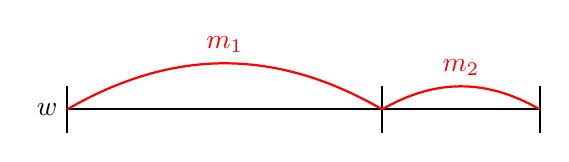
\begin{tikzpicture}
      \coordinate (A) at (0,0);
      \coordinate (B) at (6,0);
      \draw[thick] (A) -- (B);
      \foreach \x in {0,4,6}{
        \coordinate (P\x) at (\x,0);
        \draw[thick] (P\x) -- ++(0,-0.3);
        \draw[thick] (P\x) -- ++(0,0.3);
      }
      \node[left] at (A) {\(w\)};
      \draw[thick, red, bend left] (A) to node[midway, above, red] {\(m_1\)} (P4);
      \draw[thick, red,bend left] (P4) to node[midway, above, red] {\(m_2\)} (P6);
    \end{tikzpicture}
  \end{figure}
  e la fattorizzazione in \(m_3m_4\) come:
  \begin{figure}[H]
    \centering
    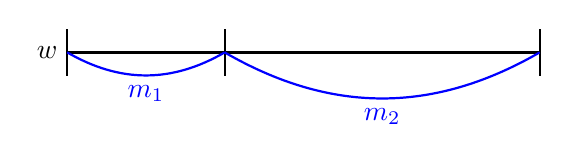
\begin{tikzpicture}
      \coordinate (A) at (0,0);
      \coordinate (B) at (6,0);
      \draw[thick] (A) -- (B);
      \foreach \x in {0,2,6}{
        \coordinate (P\x) at (\x,0);
        \draw[thick] (P\x) -- ++(0,-0.3);
        \draw[thick] (P\x) -- ++(0,0.3);
      }
      \node[left] at (A) {\(w\)};
      \draw[thick, blue,bend right] (A) to node[midway, below, blue] {\(m_1\)} (P2);
      \draw[thick, blue,bend right] (P2) to node[midway, below, blue] {\(m_2\)} (P6);
    \end{tikzpicture}
  \end{figure}
  Se \(\abs{m_1} = \abs{m_3}\), dall'ipotesi che \(M\) è libero segue che \(m_1 = m_3\) e \(m_2 = m_4\).
  Questo perché, non fossero uguali, si avrebbe una doppia fattorizzazione di \(w\), in contraddizione con la definizione di base.
  Il teorema in questo caso è verificato ponendo \(v = \varepsilon\).

  Nel caso \(\abs{m_1} > \abs{m_3}\) invece, il punto di divisione tra \(m_1\) e \(m_2\) si trova a destra del punto di divisione tra \(m_3\) e \(m_4\).
  Di conseguenza, è possibile sovrapporre le rappresentazioni precedenti come segue:
  \begin{figure}[H]
    \centering
    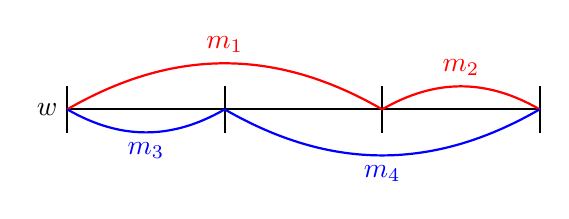
\begin{tikzpicture}
      \coordinate (A) at (0,0);
      \coordinate (B) at (6,0);
      \draw[thick] (A) -- (B);
      \foreach \x in {0,2,4,6}{
        \coordinate (P\x) at (\x,0);
        \draw[thick] (P\x) -- ++(0,-0.3);
        \draw[thick] (P\x) -- ++(0,0.3);
      }
      \node[left] at (A) {\(w\)};
      \draw[thick, red, bend left] (A) to node[midway, above, red] {\(m_1\)} (P4);
      \draw[thick, red,bend left] (P4) to node[midway, above, red] {\(m_2\)} (P6);
      \draw[thick, blue,bend right] (A) to node[midway, below, blue] {\(m_3\)} (P2);
      \draw[thick, blue,bend right] (P2) to node[midway, below, blue] {\(m_4\)} (P6);
    \end{tikzpicture}
  \end{figure}
  Chiamando \(v\) la parola compresa tra i due punti di divisione si ha che \(m_1 = m_3v\) e \(vm_2 = m_4\).
  Anche in questo caso, se una delle due uguaglianze non fosse verificata, si avrebbe una doppia fattorizzazione di \(w\), in contraddizione con la definizione di base.
  \begin{figure}
    \centering
    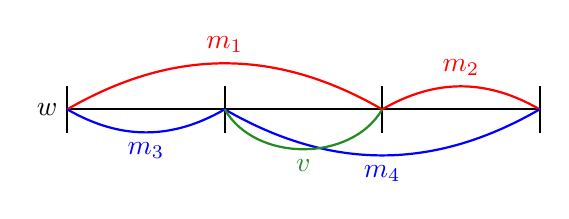
\begin{tikzpicture}
      \coordinate (A) at (0,0);
      \coordinate (B) at (6,0);
      \draw[thick] (A) -- (B);
      \foreach \x in {0,2,4,6}{
        \coordinate (P\x) at (\x,0);
        \draw[thick] (P\x) -- ++(0,-0.3);
        \draw[thick] (P\x) -- ++(0,0.3);
      }
      \node[left] at (A) {\(w\)};
      \draw[thick, red, bend left] (A) to node[midway, above, red] {\(m_1\)} (P4);
      \draw[thick, red,bend left] (P4) to node[midway, above, red] {\(m_2\)} (P6);
      \draw[thick, blue,bend right] (A) to node[midway, below, blue] {\(m_3\)} (P2);
      \draw[thick, blue,bend right] (P2) to node[midway, below, blue] {\(m_4\)} (P6);
      \draw[thick, ForestGreen, bend right=60] (P2) to node[midway, below, ForestGreen] {\(v\)} (P4);
    \end{tikzpicture}
  \end{figure}
  
  
\end{proof}

\begin{definition}[Insiemi quoziente]\label{def:quotien_set}
  Siano \(Y,Z \subseteq M\) monoide. Definiamo gli insieme quoziente destro e sinistro come:
  \begin{equation}
    \begin{aligned}
      Y^{-1}Z &= \set{m \in M}[ \exists y \in Y, ym \in Z] = \set{m \in M}[Y\set{m} \cap Z \neq \emptyset]\\
      ZY^{-1} &= \set{m \in M}[ \exists y \in Y, my \in Z] = \set{m \in M}[\set{m}Y \cap Z \neq \emptyset]
    \end{aligned}
  \end{equation}
\end{definition}

In altre parole possiamo vedere l'insieme quoziente sinistro (rispettivamente destro) come l'insieme delle parole di \(M\) che servono a completare a sinistra (rispettivamente destra) una parola di \(Y\) per ottenere una parola di \(Z\).

Utilizzando tali insieme è possibile formulare un importate teorema sui sottomonoidi liberi.

\begin{theorem}[Schuïtzenberger]\label{thm:schuïtzenberger}
  Sia \(M\) libero e \(N \leq M\). Allora \(N \text{ è libero } \iff N^{-1}N \cap NN^{-1} \subseteq N\)
\end{theorem}
In altre parole questo teorema ci dice che \(N\) sottomonoide di \(M\) libero è a sua volta libero se e solo se ogni parola di \(M\) che completa sia a destra che a sinistra parole di \(N\) sia a sua volta inclusa in \(N\).
Tale formulazione può essere espressa formalmente come:
\[N \text{ libero } \iff \left(\forall m \in M (\exists n_1,n_2,n_3,n_4( n_1m=n_2 \land mn_3=n_4) \implies m \in N)\right)\]

Per dare un idea del perché di questo risultato possiamo ragionare per assurdo, considerando l'ipotesi che esista \(m \in M\) che completa sia a sinistra che a destra parole di \(N\) senza appartenere esso stesso a \(N\).
Prendendo allora per esempio il caso \(n_1m=n_2\) si avrà che o le parole della base di \(M\) che compongono \(m\) appartengono a \(N\) ma senza formare \(m\) stesso, e dunque \(N\) non è libero, o tali parole non appartengono a \(N\) e dunque deve esistere in \(n' \in N\st n_1n'=n_2\) con \(n' \neq m\).
Essendo però queste tutte parole anche di \(M\), si avrebbe che \(n_2 \in M\), e in particolare il suo resto da \(n_1\) ha una doppia fattorizzazione.
\todo{Chiedere a De Luca se e sufficiente come dim, e se si a che serve che \(m\) sia quoto sia sinistro che destro, in questo ragionamento basta solo un lato.}

\begin{note}[Osservazioni]
  Se \(N\leq M\) necessariamente \(N \subseteq N^{-1}N \cap NN^{-1}\) poiché tutte le parole di \(N\) completano sia a destra che a sinistra la parola vuota per formare se stesse.
  Di conseguenza il teorema può essere riformulato equivalentemente come:
  \begin{theorem}[Schuïtzenberger alt.]
    Sia \(M\) libero e \(N \leq M\). Allora \(N \text{ è libero } \iff N^{-1}N \cap NN^{-1} = N\)
  \end{theorem}
  In altre parole un sottomonoide di un monoide libero è esso stesso libero se non contiene più del necessario.
\end{note}
  \todo{Chiedere esempio di \(N \leq M\) non libero con \(M\) libero}

\begin{definition}[Sottomoide unitario]
  Dato \(M\) monoide, \(N \leq M\) è detto \keyword{unitario a sinistra} (rispettivamente a destra) se:
  \[N^{-1}N \subseteq N \text{ sx}\]
  \[NN^{-1} \subseteq N \text{ dx}\]
  \(N\) si dice \keyword{unitario} se è unitario a sinistra o a destra.
\end{definition}

Da tale definizione e dal teorema~\ref{thm:schuïtzenberger} segue che, dato \(M\) monoide libero, se \(N \leq M\) è libero, allora è unitario.

